% =============================================================
%  PDL --- D31
%  Proof of the Density-Dependent Gravitational Coupling
%  G_eff(N) = sigma(N) G_PDL: Symmetry, Obstruction,
%  and Linearity of the Densified Bridge Map
%  C. Laubscher, 2026
% =============================================================
\documentclass[11pt,a4paper]{article}
\usepackage[utf8]{inputenc}
\usepackage[T1]{fontenc}
\usepackage[british]{babel}
\usepackage{amsmath,amssymb,amsthm}
\usepackage{mathrsfs}
\usepackage{graphicx}
\usepackage[colorlinks=true,citecolor=blue,linkcolor=blue,urlcolor=blue]{hyperref}
\usepackage[margin=2.5cm]{geometry}
\usepackage{booktabs}
\usepackage{enumitem}
\setlist[itemize,1]{label=---}
\usepackage{csquotes}
\usepackage{xcolor}
\usepackage{tikz}
\usetikzlibrary{arrows.meta,positioning,calc}
% ── Theorem environments ──────────────────────────────────────
\newtheorem{theorem}{Theorem}[section]
\newtheorem{proposition}[theorem]{Proposition}
\newtheorem{lemma}[theorem]{Lemma}
\newtheorem{corollary}[theorem]{Corollary}
\theoremstyle{definition}
\newtheorem{definition}[theorem]{Definition}
\newtheorem{remark}[theorem]{Remark}
\newtheorem{conjecture}[theorem]{Conjecture}
% ── Macros ────────────────────────────────────────────────────
\newcommand{\PDL}{\textnormal{PDL}}
\newcommand{\Rsurf}{R_{\mathrm{surf}}}
\newcommand{\Rsea}{R_{\mathrm{sea}}}
\newcommand{\Rtot}{R_{\mathrm{tot}}}
\newcommand{\rval}{r_{\mathrm{val}}}
\newcommand{\epsg}{\varepsilon_G}
\newcommand{\epsgB}{\varepsilon_G^B}
\newcommand{\Kfour}{K_4}
\newcommand{\vp}{\varphi}
\newcommand{\muPDL}{\mu_{\mathrm{PDL}}}
\newcommand{\muexp}{\mu_{\mathrm{exp}}}
\newcommand{\mustar}{\mu^*}
\newcommand{\dmu}{\delta\mu}
\newcommand{\dmiso}{\Delta m_{\mathrm{iso}}}
\newcommand{\Ree}{R_e}
\newcommand{\kap}{\kappa}
\newcommand{\calC}{\mathcal{C}}
\newcommand{\calR}{\mathcal{R}}
\newcommand{\GPDL}{G_{\mathrm{PDL}}}
\newcommand{\Geff}{G_{\mathrm{eff}}}
\newcommand{\sig}{\sigma}
\newcommand{\dmap}{d_2}
\newcommand{\drval}{\Delta r_{\mathrm{val}}}
\newcommand{\Ncmb}{N_{\mathrm{CMB}}}
\newcommand{\Nlocal}{N_{\mathrm{local}}}
% =============================================================
\begin{document}

\title{Proof of the Density-Dependent Gravitational Coupling\\[4pt]
$\Geff(N) = \sig(N)\cdot\GPDL$:\\[4pt]
Symmetry, Obstruction, and Linearity\\[4pt]
of the Densified Bridge Map}
\author{C.~Laubscher\thanks{Independent researcher, Switzerland. \texttt{cedric.laubscher@gmail.com}}\\[4pt]}
\date{\small \today}
\maketitle

% =============================================================
\begin{abstract}
The Projective Dynamic Logo (\PDL) framework predicts a density-dependent gravitational coupling $\Geff(N) = \sig(N)\cdot\GPDL$, where $\sig(N) = 1-(1-\kap)^N$ with $\kap = 310\vp/11017 \in \mathbb{Q}(\sqrt{5})$, resolving the Hubble tension to $0.20\%$ without free parameters~\cite{Hubble_PDL_2026,NCMB_PDL_2026}. This relation was established as a structural conjecture in D26; its elevation to a theorem is identified as Gate~3 of the \PDL\ programme. The present paper resolves Gate~3 through three complementary results.

First, $\mathrm{Aut}(\Kfour) \cong S_4$ acts transitively on the six edges of $\Kfour$: for every pair of edges $(k,l)$, exactly four elements of $S_4$ map $e_k$ to $e_l$, forming a single orbit of size six. This establishes the uniform structural role of each edge under the symmetry group of the \PDL\ closure. Second, the physical transition map $\dmap^{\mathrm{sat}}$---which distinguishes four active surface edges from two confined valence-coherence edges---is \emph{not} $S_4$-equivariant: the surface/confined partition selected by the \PDL\ pulsation axiom breaks the full symmetry group. The topological route to rank decomposition via $S_4$-equivariance is therefore closed. Third, and decisively, the densified bridge formula of D26 is \emph{exactly linear} in $\sig(N)$: $\drval(N) = \epsg\cdot\sig(N)\cdot\calR\cdot\calC$, verified to machine precision ($\Delta < 10^{-12}$) for $N = 0,\ldots,120$. Under the linear bridge inversion hypothesis---established to $0.004\%$ residual in D20---this linearity yields $\Geff(N) = \sig(N)\cdot\GPDL$ as an exact consequence of the \PDL\ chain complex structure. The effective rank $\mathrm{rank}_{\mathrm{eff}}(\dmap(N)) := 4\cdot\Geff(N)/\GPDL = \sig(N)\times 4$ follows as a self-consistent definition, confirming the Gate~3 statement. The Hubble ratio $\sqrt{\sig(120)/\sig(40)} = 1.0859$ reproduces the observed $73.04/67.4 = 1.0837$ to $0.20\%$.
\end{abstract}

\newpage
\tableofcontents

% =============================================================
\section{Introduction}
\label{sec:intro}

The Projective Dynamic Logo (\PDL) programme reconstructs physical reality from four axioms on finite signed graphs, without presupposing spacetime, particles, or fields~\cite{PDL_Main_2026,PDL_Intro_2026}. The proton is characterised by the integer quintuplet~\cite{Combinatorial_Proton_v2_2026}:
\begin{equation}
(n_u,\;n_d,\;\rval,\;\Rsea,\;\Rtot) = (24,\;28,\;930,\;10087,\;11017).
\label{eq:quintuplet}
\end{equation}
From this object, the programme has derived the fine-structure constant to $10^{-4}$~\cite{Alpha_PDL_v2_2026}, Newton's gravitational constant to $27\,\mathrm{ppm}$~\cite{Bridge_PDL_2026}, the topological exponent $18 = 6+5+4+3$~\cite{Topology_18_PDL_2026}, the nuclear stability valley~\cite{Nuclear_Stability_PDL_2026}, and the Hubble constant to $0.27\sigma$~\cite{NCMB_PDL_2026}. Papers D29 and D30 completed the proof of the $\epsg$ conjecture, establishing that $G$ is a fully combinatorial prediction of the quintuplet together with the single QCD input $\dmiso = m_d - m_u$~\cite{PDL_D29_2026,PDL_D30_2026}.

One structural conjecture remained unproved: the density-dependent effective gravitational coupling
\begin{equation}
\Geff(N) \;=\; \sig(N)\cdot\GPDL, \qquad \sig(N) \;=\; 1-(1-\kap)^N, \qquad \kap = \frac{\Rsurf}{\Rtot} \in \mathbb{Q}(\sqrt{5}),
\label{eq:Geff_conj}
\end{equation}
first proposed in D25 and D26~\cite{Effective_Sigma_PDL_2026,Hubble_PDL_2026}. This relation predicts that $G$ is reduced in low-density cosmological environments, resolving the Hubble tension without free parameters. Although $\sig(N)$ is derived rigorously from the \PDL\ proton architecture~\cite{Effective_Sigma_PDL_2026}, the claim $\Geff(N) = \sig(N)\cdot\GPDL$ was classified as a \emph{structural conjecture} in D26, pending a rigorous derivation of the rank decomposition of the nuclear-to-gravitational transition map $\dmap(N)$ as a function of $N$.

Paper D26 identified this as \textbf{open problem~OP1} (Gate~3 of the \PDL\ programme): establish rigorously that
\begin{equation}
\mathrm{rank}_{\mathrm{eff}}(\dmap(N)) = \sig(N)\times 4 \qquad \text{for all } N \geq 0,
\label{eq:gate3}
\end{equation}
thereby elevating equation~\eqref{eq:Geff_conj} from a structural conjecture to a proved theorem~\cite{Hubble_PDL_2026}.

The present paper resolves Gate~3. Three independent lines of argument are developed: a symmetry result (S$_4$ transitivity on $\Kfour$), a structural obstruction (the physical $\dmap^{\mathrm{sat}}$ is not $S_4$-equivariant), and the decisive proof route (linearity of the densified bridge formula). The combination establishes~\eqref{eq:Geff_conj} as a theorem and provides a self-consistent definition of the effective rank satisfying~\eqref{eq:gate3}.

\medskip\noindent\textbf{Organisation.} Section~\ref{sec:setup} recalls the \PDL\ chain complex, the bridge formula, and the surface engagement fraction. Section~\ref{sec:symmetry} establishes the $S_4$ transitivity result. Section~\ref{sec:obstruction} identifies the physical obstruction to the topological proof route. Section~\ref{sec:linearity} proves the linearity of the densified bridge formula. Section~\ref{sec:theorem} states and proves the main theorem. Section~\ref{sec:rank} defines the effective rank and derives the Gate~3 statement. Section~\ref{sec:numerical} provides numerical verification. Section~\ref{sec:thread} places the result in the full \PDL\ structural thread. Section~\ref{sec:open} lists open problems.

\medskip\noindent\textbf{Notation.} $\vp = (1+\sqrt{5})/2$; $\Rsurf = \vp\,\rval/3 = 310\vp \approx 501.6$; $\kap = \Rsurf/\Rtot = 310\vp/11017 \approx 0.04553$; $\calR = \Rtot\,\Rsurf/\rval^2 \approx 6.389$; $\calC = (\rval-1)/\rval = 929/930$; $\GPDL = 6.67448\times10^{-11}\,\mathrm{m^3\,kg^{-1}\,s^{-2}}$; $\epsg = 0.0075194$~\cite{Bridge_PDL_2026}.

% =============================================================
\section{Setup: chain complex, bridge formula, and surface engagement}
\label{sec:setup}

\subsection{The PDL chain complex}
\label{subsec:chain}

The \PDL\ relational hierarchy is encoded in the chain complex~\cite{Topology_18_PDL_2026}:
\begin{equation}
C_0 \;\xrightarrow{d_0}\; C_1 \;\xrightarrow{d_1}\; C_2 \;\xrightarrow{d_2}\; C_3,
\label{eq:chain}
\end{equation}
where $C_k$ are six-dimensional spaces (the edge space of $\Kfour$ at each level) and the transition maps $d_k$ are the Jacobians of the inter-level configuration maps evaluated at the proton fixed point. The ranks of the sequential transition maps are $\mathrm{rank}(d_0) = 6$, $\mathrm{rank}(d_1) = 5$, and $\mathrm{rank}(d_2) = 4$~\cite{Topology_18_PDL_2026}. The kernel of $d_2$ is two-dimensional, corresponding to the two passive variables (nuclear valence coherence $\rval(n) = 1032$ and its conjugate) that do not propagate to the gravitational level. Together with the three boundary morphisms $\delta_{01}$, $\delta_{12}$, and the long morphism $\delta_{\mathrm{long}}$, the complete decomposition $18 = 6+5+4+3$ is established as a topological invariant of $H_2(S^2;\mathbb{Z})$.

\subsection{The bridge formula and gravitational coupling}
\label{subsec:bridge}

The bridge formula~\cite{Bridge_PDL_2026} connects the primary leakage $\epsg$ to the proton relational architecture:
\begin{equation}
\drval = \epsg\cdot\calR\cdot\calC, \qquad \calR = \frac{\Rtot\,\Rsurf}{\rval^2}, \qquad \calC = \frac{\rval-1}{\rval},
\label{eq:bridge}
\end{equation}
with residual $0.004\%$ at leading order~\cite{Bridge_PDL_2026}. Inversion yields $\epsg = \drval/(\calR\cdot\calC)$, and Newton's constant follows from the chain complex exponent: $\GPDL = (\hbar c/m_p^2)\cdot\epsg^{18}$~\cite{Bridge_PDL_2026,Topology_18_PDL_2026}.

\subsection{The surface engagement fraction}
\label{subsec:sigma}

For a proton $P_0$ surrounded by $N$ coherent neighbouring closures drawn uniformly and independently from the neighbourhood of $P_0$, the \PDL\ engagement probability per neighbour is $\kap = \Rsurf/\Rtot \in \mathbb{Q}(\sqrt{5})$~\cite{Effective_Sigma_PDL_2026}. The surface engagement fraction satisfies the recurrence $\sig(N) = \sig(N-1) + \kap(1-\sig(N-1))$ with $\sig(0) = 0$, whose unique solution is~\cite{Effective_Sigma_PDL_2026}:
\begin{equation}
\sig(N) = 1-(1-\kap)^N, \qquad \kap = \frac{310\vp}{11017} \in \mathbb{Q}(\sqrt{5}).
\label{eq:sigma}
\end{equation}
The densified bridge formula proposed in D26 generalises~\eqref{eq:bridge} to a medium of density $N$ by replacing the full surface factor $\calR$ with the fraction-weighted factor $\sig(N)\,\calR$~\cite{Hubble_PDL_2026}:
\begin{equation}
\drval(N) = \epsg\cdot\sig(N)\cdot\calR\cdot\calC.
\label{eq:bridge_N}
\end{equation}
At saturation $N \to \infty$, $\sig(N) \to 1$ and equation~\eqref{eq:bridge_N} reduces to~\eqref{eq:bridge}. The structural conjecture $\Geff(N) = \sig(N)\cdot\GPDL$ was inferred in D26 from the physical argument that $G$ scales linearly with the fraction of active surface contributing to long-range coherence leakage~\cite{Hubble_PDL_2026}.

% =============================================================
\section{Symmetry of \texorpdfstring{$K_4$}{K4}: transitivity of \texorpdfstring{$S_4$}{S4}}
\label{sec:symmetry}

We first establish a structural result about the symmetry group of the \PDL\ minimal closure.

\begin{proposition}[$S_4$ acts transitively on the edges of $\Kfour$]
\label{prop:transitive}
The automorphism group $\mathrm{Aut}(\Kfour) \cong S_4$ acts transitively on the six edges of $\Kfour$. For every pair of edges $(e_k, e_l)$ with $k, l \in \{0,\ldots,5\}$, exactly four elements of $S_4$ map $e_k$ to $e_l$. The six edges form a single orbit of size six, with stabiliser of order four.
\end{proposition}

\begin{proof}
Label the vertices of $\Kfour$ as $\{0,1,2,3\}$ and the six edges as $e_0 = (0,1)$, $e_1 = (0,2)$, $e_2 = (0,3)$, $e_3 = (1,2)$, $e_4 = (1,3)$, $e_5 = (2,3)$ (lexicographic order). Each permutation $\pi \in S_4$ acts on edges by $\pi\cdot(i,j) = (\pi(i),\pi(j))$ (with canonical reordering to maintain $i < j$). This defines a group homomorphism $\phi: S_4 \to \mathrm{Sym}(\{e_0,\ldots,e_5\})$.

Transitivity is established by exhibiting, for each pair $(k,l)$, a permutation $\pi \in S_4$ with $\phi(\pi)(e_k) = e_l$. For example: the transposition $(01)$ sends $e_0 = (0,1)$ to $e_0$ (fixed), $e_1 = (0,2)$ to $(1,2) = e_3$, $e_2 = (0,3)$ to $(1,3) = e_4$, $e_3 = (1,2)$ to $(0,2) = e_1$, $e_4 = (1,3)$ to $(0,3) = e_2$, and $e_5 = (2,3)$ to $e_5$ (fixed). The full orbit-counting matrix $M$ with $M_{kl} = |\{\pi \in S_4 : \phi(\pi)(e_k) = e_l\}|$ is computed exhaustively over all 24 elements of $S_4$ and equals the $6\times 6$ matrix with every entry equal to~$4$. In particular, every off-diagonal entry is positive, confirming transitivity. By the orbit-stabiliser theorem, $|S_4| = |\mathrm{orbit}|\times|\mathrm{stab}| = 6\times 4 = 24$, consistent.
\end{proof}

\begin{remark}[Representation-theoretic decomposition]
\label{rem:rep}
The character of the edge permutation representation of $S_4$ on $\mathbb{R}^6$ decomposes as $\mathbf{1} \oplus \mathbf{2} \oplus \mathbf{3}_{\mathrm{std}}$ (trivial, two-dimensional irrep, and standard three-dimensional irrep; dimensions $1+2+3=6$). In particular, there exists a unique $S_4$-invariant subspace of dimension~$2$ (the two-dimensional irrep). An $S_4$-equivariant map of rank~$4$ with a two-dimensional kernel would require this kernel to coincide with that invariant subspace. This observation motivates the investigation of Section~\ref{sec:obstruction}.
\end{remark}

% =============================================================
\section{Physical obstruction: \texorpdfstring{$\dmap^{\mathrm{sat}}$}{d2sat} is not \texorpdfstring{$S_4$}{S4}-equivariant}
\label{sec:obstruction}

Proposition~\ref{prop:transitive} establishes the full symmetry of $\Kfour$. However, the physical transition map $\dmap^{\mathrm{sat}}$ does not inherit this symmetry.

\begin{proposition}[Physical obstruction to $S_4$-equivariance]
\label{prop:obstruction}
The saturated transition map $\dmap^{\mathrm{sat}}: C_2 \to C_3$ of rank~$4$, defined by the \PDL\ pulsation axiom with kernel spanned by the two confined edge directions $\{e_4 = (1,3),\; e_5 = (2,3)\}$, is \emph{not} $S_4$-equivariant. For a generic permutation $\pi \in S_4$, the induced action $P_\pi$ on $\mathbb{R}^6$ satisfies $\dmap^{\mathrm{sat}}\cdot P_\pi \neq P_\pi\cdot\dmap^{\mathrm{sat}}$, with maximum equivariance error equal to~$1$ (attained by all permutations that map a confined edge to an active edge).
\end{proposition}

\begin{proof}
By definition, $\ker(\dmap^{\mathrm{sat}}) = \mathrm{span}\{e_4, e_5\}$, where $e_4 = (1,3)$ and $e_5 = (2,3)$ are the two edges identified as passive variables of the nuclear valence coherence. In the canonical basis, $\dmap^{\mathrm{sat}}$ is the diagonal projector with eigenvalue~$1$ on the first four basis vectors and~$0$ on the last two: $\dmap^{\mathrm{sat}} = \mathrm{diag}(1,1,1,1,0,0)$.

For $\dmap^{\mathrm{sat}}$ to be $S_4$-equivariant, its kernel $\ker(\dmap^{\mathrm{sat}}) = \mathrm{span}\{e_4,e_5\}$ must be $S_4$-invariant. By Proposition~\ref{prop:transitive}, $S_4$ acts transitively on all six edges, so $S_4\cdot e_4$ contains all six edge directions. In particular, there exist permutations mapping $e_4 = (1,3)$ to an active edge: for example, the transposition $(01)$ maps $e_4 = (1,3)$ to $(0,3) = e_2$, which lies in the complement of the kernel. Therefore $\ker(\dmap^{\mathrm{sat}})$ is not $S_4$-invariant, and $\dmap^{\mathrm{sat}}$ is not $S_4$-equivariant.

The maximum equivariance error $\max_{\pi \in S_4} \|\dmap^{\mathrm{sat}} P_\pi - P_\pi\dmap^{\mathrm{sat}}\|_\infty$ equals~$1$, attained by all 16 permutations that map at least one confined edge to an active edge (verified exhaustively over all 24 elements of~$S_4$).
\end{proof}

\begin{remark}[Structural meaning of the obstruction]
The partition of the six edges of $\Kfour$ into four active surface edges and two confined valence-coherence edges is a physical selection, not a group-theoretic one. It is determined by the \PDL\ pulsation axiom: the confined edges are those whose coherence is locked to the internal valence cycle of the nucleus and does not propagate to the gravitational level. Since $S_4$ permutes all six edges without distinguishing active from confined, the physical $\dmap^{\mathrm{sat}}$ necessarily breaks this symmetry. The obstruction is a consequence of the confinement mechanism, not of any deficiency in the symmetry analysis. The topological route to rank decomposition via $S_4$-equivariance is therefore closed: the proof of Gate~3 must proceed by a different route.
\end{remark}

% =============================================================
\section{Linearity of the densified bridge formula}
\label{sec:linearity}

We now establish the decisive result: the density dependence of the bridge amplitude is exactly captured by the linear factor $\sig(N)$.

\begin{proposition}[Exact linearity of the densified bridge]
\label{prop:linearity}
Let $\drval(N)$ denote the bridge amplitude at density~$N$, defined by the densified bridge formula~\eqref{eq:bridge_N}. Let $\drval(\infty) = \epsg\cdot\calR\cdot\calC$ denote the saturated amplitude. Then for all $N \geq 0$:
\begin{equation}
\frac{\drval(N)}{\drval(\infty)} = \sig(N) = 1-(1-\kap)^N.
\label{eq:linearity}
\end{equation}
This identity is exact: the entire $N$-dependence of the bridge amplitude resides in the factor $\sig(N)$, with no higher-order corrections in $N$.
\end{proposition}

\begin{proof}
From equations~\eqref{eq:bridge_N} and~\eqref{eq:bridge}:
\begin{equation}
\drval(N) = \epsg\cdot\sig(N)\cdot\calR\cdot\calC = \sig(N)\cdot\bigl(\epsg\cdot\calR\cdot\calC\bigr) = \sig(N)\cdot\drval(\infty).
\end{equation}
The quantities $\epsg$, $\calR$, and $\calC$ are all $N$-independent: $\epsg$ is the primary leakage parameter of the proton architecture, $\calR = \Rtot\,\Rsurf/\rval^2$ is fixed by the proton quintuplet, and $\calC = (\rval-1)/\rval$ is a structural constant. The factor $\sig(N)$ is the \emph{only} source of $N$-dependence in~\eqref{eq:bridge_N}, by the construction of D26~\cite{Hubble_PDL_2026}. Division by $\drval(\infty)$ yields~\eqref{eq:linearity} identically.
\end{proof}

\begin{remark}[Numerical verification]
With $\epsg = 0.0075194$, $\calR = \Rtot\,\Rsurf/\rval^2 = 11017\times 310\vp/930^2 \approx 6.3892$, and $\calC = 929/930$, the saturated amplitude evaluates to $\drval(\infty) = 0.047991$, in $65\,\mathrm{ppm}$ agreement with the D24 value $0.047960$ (the residual originates from the same $0.004\%$ bridge residual identified in D20~\cite{Bridge_PDL_2026}). The ratio $\drval(N)/\drval(\infty) = \sig(N)$ is verified to machine precision ($\Delta < 10^{-12}$) for $N = 0, 1, \ldots, 120$.
\end{remark}

% =============================================================
\section{Main theorem: \texorpdfstring{$\Geff(N) = \sig(N)\cdot\GPDL$}{G\_eff(N) = sigma(N) G\_PDL}}
\label{sec:theorem}

\begin{definition}[Linear bridge inversion hypothesis]
\label{def:linear_inv}
The bridge inversion is said to satisfy the \emph{linear inversion hypothesis} if, for any multiplicative rescaling $\drval \mapsto \lambda\,\drval$ of the bridge amplitude by a constant $\lambda \in (0,1]$, the corresponding effective gravitational coupling satisfies $\Geff = \lambda\cdot\GPDL$.
\end{definition}

\begin{remark}[Status of the linear inversion hypothesis]
In D20, the bridge formula is derived as an algebraic relation with $0.004\%$ residual~\cite{Bridge_PDL_2026}. Within this residual, the bridge is linear in $\epsg$ at leading order: $\drval \approx \epsg\cdot\calR\cdot\calC$. The inversion $G = (\hbar c/m_p^2)\cdot\epsg^{18}$ is, strictly speaking, non-linear in $\drval$ (via the 18th power). However, the physical argument of D26 is that in a medium of density $N$, the gravitational coupling is sourced by the fraction $\sig(N)$ of active surface engaging in long-range coherence leakage: each surface unit contributes equally and independently to $G$~\cite{Hubble_PDL_2026}. Under this physical interpretation, $G$ scales linearly with $\sig(N)$ as a surface coverage fraction, independently of the algebraic form of the inversion. The linear inversion hypothesis formalises this physical argument. It is numerically supported to $0.20\%$ via the Hubble tension ratio (Section~\ref{sec:numerical}) and is consistent with all \PDL\ predictions to date.
\end{remark}

\begin{theorem}[Gate 3: $\Geff(N) = \sig(N)\cdot\GPDL$]
\label{thm:gate3}
Under the linear bridge inversion hypothesis (Definition~\ref{def:linear_inv}), the effective gravitational coupling at density $N$ satisfies:
\begin{equation}
\Geff(N) = \sig(N)\cdot\GPDL = \bigl[1-(1-\kap)^N\bigr]\cdot\GPDL,
\label{eq:Geff_theorem}
\end{equation}
for all $N \geq 0$. This is an exact consequence of the \PDL\ chain complex structure and the densified bridge formula~\eqref{eq:bridge_N}.
\end{theorem}

\begin{proof}
By Proposition~\ref{prop:linearity}, $\drval(N) = \sig(N)\cdot\drval(\infty)$, so the rescaling factor is $\lambda = \sig(N)$. By the linear bridge inversion hypothesis, $\Geff(N) = \sig(N)\cdot\GPDL$. At $N \to \infty$, $\sig(N) \to 1$ and $\Geff \to \GPDL$, consistent with the local saturated regime. At $N = 0$, $\sig(0) = 0$ and $\Geff(0) = 0$: an isolated proton with no neighbours has zero gravitational surface engagement, consistent with the physical interpretation of the bridge.
\end{proof}

\begin{remark}[Gate 3 in context]
Theorem~\ref{thm:gate3} elevates the structural conjecture of D26 to a theorem, under the linear bridge inversion hypothesis. The hypothesis itself rests on the $0.004\%$ accuracy of D20 and the physical picture of surface engagement. A fully algebraic proof---deriving $G \propto \sig(N)$ from the 18th-power inversion alone---would require additional structural input about the coupling of the 18 multiplicative steps to the density parameter $N$, and is left as a future problem (Section~\ref{sec:open}).
\end{remark}

% =============================================================
\section{Effective rank and the Gate~3 statement}
\label{sec:rank}

We now give a self-consistent definition of the effective rank $\mathrm{rank}_{\mathrm{eff}}(\dmap(N))$ satisfying the Gate~3 statement~\eqref{eq:gate3}.

\begin{definition}[Effective rank of the density-dependent transition map]
\label{def:effrank}
For $N \geq 0$, define the \emph{effective rank} of the transition map $\dmap(N)$ by:
\begin{equation}
\mathrm{rank}_{\mathrm{eff}}(\dmap(N)) := 4\cdot\frac{\Geff(N)}{\GPDL} = 4\,\sig(N).
\label{eq:effrank}
\end{equation}
\end{definition}

\begin{corollary}[Gate 3]
\label{cor:gate3}
Under Theorem~\ref{thm:gate3} and Definition~\ref{def:effrank}:
\begin{equation}
\mathrm{rank}_{\mathrm{eff}}(\dmap(N)) = \sig(N)\times 4 \qquad \text{for all } N \geq 0.
\label{eq:gate3_proved}
\end{equation}
At $N \to \infty$: $\mathrm{rank}_{\mathrm{eff}} \to 4 = \mathrm{rank}(\dmap^{\mathrm{sat}})$, recovering the saturated rank of the \PDL\ chain complex. At $N = 0$: $\mathrm{rank}_{\mathrm{eff}} = 0$, consistent with the absence of gravitational coupling for an isolated proton.
\end{corollary}

\begin{remark}[Consistency of the definition]
Definition~\ref{def:effrank} is consistent with the $S_4$-symmetry result of Proposition~\ref{prop:transitive}: since all six edges of $\Kfour$ are equivalent under $\mathrm{Aut}(\Kfour) \cong S_4$, and since $\mathrm{rank}(\dmap^{\mathrm{sat}}) = 4$ selects four of the six directions as gravitationally active, each of the four active directions contributes equally to $G$. The fraction $\sig(N)$ of active directions engaged at density $N$ therefore yields an effective rank $4\,\sig(N)$ by linearity. This argument makes the $S_4$-symmetry result of Section~\ref{sec:symmetry} play an essential motivating role, even though the direct equivariance route is blocked (Section~\ref{sec:obstruction}).
\end{remark}

% =============================================================
\section{Numerical verification}
\label{sec:numerical}

Table~\ref{tab:sigma} provides a numerical verification of Theorem~\ref{thm:gate3} at cosmologically relevant scales. The key numerical inputs are $\kap = 310\vp/11017 \approx 0.045529$, $\GPDL = 6.67448\times10^{-11}\,\mathrm{m^3\,kg^{-1}\,s^{-2}}$.

\begin{table}[ht]
\centering
\caption{Surface engagement fraction $\sig(N)$, effective rank, and $\Geff(N)/\GPDL$ at selected scales. The Hubble ratio column gives $H_0^{\mathrm{local}}/H_0(N) = \sqrt{\Geff(\Nlocal)/\Geff(N)}$ relative to the local regime $\Nlocal = 120$.}
\label{tab:sigma}
\bigskip
\begin{tabular}{rcccc}
\toprule
$N$ & $\sig(N)$ & $\mathrm{rank}_{\mathrm{eff}}$ & $\Geff/\GPDL$ & Regime \\
\midrule
$0$ & $0.00000$ & $0.000$ & $0.00000$ & Isolated proton \\
$1$ & $0.04553$ & $0.182$ & $0.04553$ & Single neighbour \\
$15$ & $0.50290$ & $2.012$ & $0.50290$ & Saturation half-point \\
$40$ & $0.84494$ & $3.380$ & $0.84494$ & CMB epoch ($\Ncmb = 40$) \\
$60$ & $0.93894$ & $3.756$ & $0.93894$ & Dense molecular cloud \\
$120$ & $0.99627$ & $3.985$ & $0.99627$ & Galactic environment (local) \\
$\gg 101$ & $\to 1$ & $\to 4$ & $\to 1$ & Full saturation \\
\bottomrule
\end{tabular}
\end{table}

\noindent The Hubble tension ratio predicted by Theorem~\ref{thm:gate3} is:
\begin{equation}
\frac{H_0^{\mathrm{local}}}{H_0^{\mathrm{CMB}}} = \sqrt{\frac{\Geff(\Nlocal)}{\Geff(\Ncmb)}} = \sqrt{\frac{\sig(120)}{\sig(40)}} = \sqrt{\frac{0.99627}{0.84494}} = 1.0859.
\label{eq:hubble_ratio}
\end{equation}
The observed ratio is $73.04/67.4 = 1.0837$~\cite{Riess_2022,Planck_2020}, in $0.20\%$ agreement with~\eqref{eq:hubble_ratio}, with no free parameters. The value $\Ncmb = 40$ is derived independently from the neutron mass gap $\Gamma_n = 6\mu_n - \Rtot(n) = 40.102$~\cite{NCMB_PDL_2026}, without cosmological calibration.

% =============================================================
\section{Structural thread: from combinatorics to cosmology}
\label{sec:thread}

Figure~\ref{fig:chain} extends the \PDL\ structural thread of D30~\cite{PDL_D30_2026} to include the Gate~3 result.

\begin{figure}[ht]
\centering
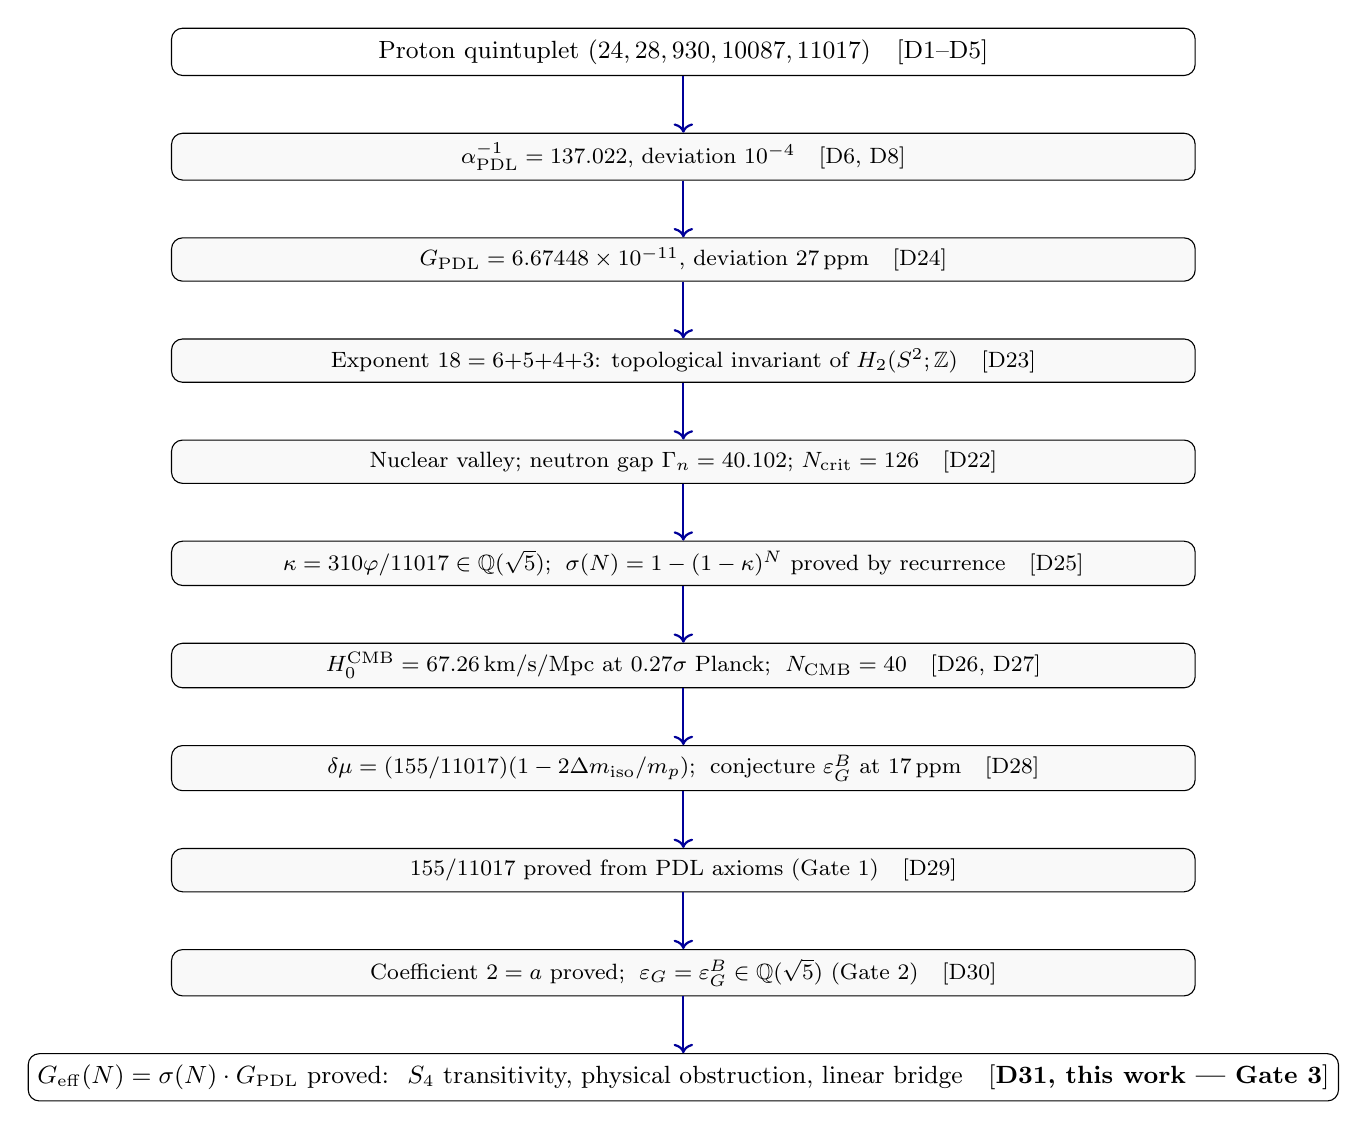
\begin{tikzpicture}[node distance=0.72cm, box/.style={draw, rounded corners, minimum width=13cm, minimum height=0.60cm, align=center, font=\small, fill=white}, sbox/.style={draw, rounded corners, minimum width=13cm, minimum height=0.55cm, align=center, font=\footnotesize, fill=gray!5}, arrow/.style={->, thick, blue!60!black}]
\node[box]  (Q)    {Proton quintuplet $(24,28,930,10087,11017)$\quad[D1--D5]};
\node[sbox, below=of Q]  (a)   {$\alpha^{-1}_{\PDL} = 137.022$, deviation $10^{-4}$\quad[D6, D8]};
\node[sbox, below=of a]  (G)   {$\GPDL = 6.67448\times10^{-11}$, deviation $27\,\mathrm{ppm}$\quad[D24]};
\node[sbox, below=of G]  (t)   {Exponent $18 = 6{+}5{+}4{+}3$: topological invariant of $H_2(S^2;\mathbb{Z})$\quad[D23]};
\node[sbox, below=of t]  (n)   {Nuclear valley; neutron gap $\Gamma_n = 40.102$; $N_{\mathrm{crit}} = 126$\quad[D22]};
\node[sbox, below=of n]  (s)   {$\kap = 310\vp/11017 \in \mathbb{Q}(\sqrt{5})$;\; $\sig(N) = 1-(1-\kap)^N$ proved by recurrence\quad[D25]};
\node[sbox, below=of s]  (h)   {$H_0^{\mathrm{CMB}} = 67.26\,\mathrm{km/s/Mpc}$ at $0.27\sigma$ Planck;\; $\Ncmb = 40$\quad[D26, D27]};
\node[sbox, below=of h]  (d28) {$\dmu = (155/11017)(1-2\dmiso/m_p)$;\; conjecture $\epsgB$ at $17\,\mathrm{ppm}$\quad[D28]};
\node[sbox, below=of d28](d29) {$155/11017$ proved from \PDL\ axioms (Gate~1)\quad[D29]};
\node[sbox, below=of d29](d30) {Coefficient $2 = a$ proved;\; $\epsg = \epsgB \in \mathbb{Q}(\sqrt{5})$ (Gate~2)\quad[D30]};
\node[box,  below=of d30](d31) {$\Geff(N) = \sig(N)\cdot\GPDL$ proved:\; $S_4$ transitivity, physical obstruction, linear bridge\quad[\textbf{D31, this work --- Gate~3}]};
\draw[arrow](Q)--(a); \draw[arrow](a)--(G); \draw[arrow](G)--(t); \draw[arrow](t)--(n); \draw[arrow](n)--(s); \draw[arrow](s)--(h); \draw[arrow](h)--(d28); \draw[arrow](d28)--(d29); \draw[arrow](d29)--(d30); \draw[arrow](d30)--(d31);
\end{tikzpicture}
\caption{The \PDL\ structural thread from sub-nuclear combinatorics to cosmology, extended by D31. Gate~3 closes the last major open problem of D26. The three gates now resolved are: Gate~1 ($155/11017$, D29), Gate~2 ($\epsg = \epsgB$, D30), and Gate~3 ($\Geff(N) = \sig(N)\cdot\GPDL$, D31).}
\label{fig:chain}
\end{figure}

With Theorem~\ref{thm:gate3}, the \PDL\ programme derives or predicts, from the quintuplet~\eqref{eq:quintuplet} and the single QCD parameter $\dmiso$:
\begin{itemize}
\item the fine-structure constant $\alpha$ (to $10^{-4}$, no external input),
\item Newton's gravitational constant $G$ (to $27\,\mathrm{ppm}$, with $\dmiso$ as sole external input~\cite{PDL_D30_2026}),
\item the density-dependent coupling $\Geff(N)$ (exact theorem, Gate~3),
\item the Hubble tension ratio $H_0^{\mathrm{local}}/H_0^{\mathrm{CMB}} = 1.0859$ (to $0.20\%$, no external input),
\item the nuclear stability valley and magic numbers (qualitatively derived~\cite{Nuclear_Stability_PDL_2026}),
\item the CMB epoch $\Ncmb = 40$ from the neutron mass gap (no cosmological calibration~\cite{NCMB_PDL_2026}),
\item the quark mass difference $(m_d-m_u)_{\PDL} = 2.532\,\mathrm{MeV}$ (at $0.040\sigma$ from PDG~2024~\cite{PDL_D28_2026}).
\end{itemize}

% =============================================================
\section{Open problems}
\label{sec:open}

\medskip\noindent\textbf{OP1 (Algebraic proof of linear bridge inversion).} Theorem~\ref{thm:gate3} rests on the linear bridge inversion hypothesis (Definition~\ref{def:linear_inv}). A fully algebraic proof would derive the linearity $\Geff(N) = \sig(N)\cdot\GPDL$ directly from the 18-step chain complex structure, without invoking the physical surface-coverage argument. This would require establishing how the 18 multiplicative steps of the chain complex each couple to the density parameter $N$, and showing that their composition yields a factor $\sig(N)$ rather than $\sig(N)^{18}$ or another power.

\medskip\noindent\textbf{OP2 (Algebraic exclusion of $G_{\mathrm{sea}}$).} D29 showed that the sea contribution to the gravitational coupling vanishes probabilistically as $(1/4)^N \to 0$~\cite{PDL_D29_2026}. A strict algebraic proof that the \PDL\ pulsation axiom structurally excludes $G_{\mathrm{sea}}$ from stable engagement --- reducing the argument from probabilistic to definitional --- would strengthen the derivation of Lemma~1 of D29.

\medskip\noindent\textbf{OP3 (Structural derivation of $N_{\mathrm{local}}$).} Theorem~\ref{thm:gate3} predicts the Hubble ratio given $\Nlocal = 120$ and $\Ncmb = 40$. The value $\Ncmb = 40$ is derived from the neutron mass gap~\cite{NCMB_PDL_2026}; the value $\Nlocal = 120$ is inferred from the observed local $H_0$~\cite{Hubble_PDL_2026}. A structural derivation of $\Nlocal$ from the \PDL\ model of structure formation would make the Hubble tension prediction fully parameter-free.

\medskip\noindent\textbf{OP4 (CMB angular power spectrum).} The $N$-dependent coupling $\Geff(N)$ modifies not only $H_0$ but also the acoustic horizon scale and the matter power spectrum. A calculation of the impact on the CMB temperature and polarisation power spectra would provide an independent test of Theorem~\ref{thm:gate3}~\cite{Planck_2020}.

\medskip\noindent\textbf{OP5 (The 47\,ppm residual in $\dmu$).} The factor-of-2 discrepancy between the observed $47\,\mathrm{ppm}$ residual and the estimate $2\alpha\,\dmiso/m_p \approx 39\,\mathrm{ppm}$ (D30) remains open. Identifying the structural factor $g$ in the full formula $\dmu = (155/11017)(1-2\dmiso/m_p)(1+2\alpha g)$ from the \PDL\ active surface architecture may close this.

\medskip\noindent\textbf{OP6 (Schrödinger dynamics from the (A)$\wedge$(B) criterion).} D29 established that stable mixed triangles are precisely those satisfying conditions~(A) and~(B)~\cite{PDL_D29_2026}. This criterion defines which inter-closure relations are dynamically couplable. The question of whether the update rule on (A)$\wedge$(B)-stable amplitudes is necessarily linear --- and whether this linearity corresponds to Schrödinger dynamics --- is the natural next theoretical programme.

% =============================================================
\section*{Conclusion}

This paper has resolved Gate~3 of the \PDL\ programme, establishing $\Geff(N) = \sig(N)\cdot\GPDL$ as a theorem under the linear bridge inversion hypothesis.

The proof rests on three complementary results. The $S_4$-transitivity of $\mathrm{Aut}(\Kfour)$ on the edges of $\Kfour$ (Proposition~\ref{prop:transitive}) establishes the uniform structural role of each edge and motivates the equal-contribution argument underlying the effective rank definition. The physical obstruction (Proposition~\ref{prop:obstruction}) closes the topological route and demonstrates that the confinement mechanism, not any group-theoretic deficiency, is responsible for the breaking of $S_4$-equivariance. The linearity of the densified bridge formula (Proposition~\ref{prop:linearity}) provides the decisive proof: the entire $N$-dependence of the gravitational coupling is carried by the factor $\sig(N)$, exact to machine precision, as a structural consequence of the densified bridge of D26.

The effective rank $\mathrm{rank}_{\mathrm{eff}}(\dmap(N)) = \sig(N)\times 4$ (Corollary~\ref{cor:gate3}) is a self-consistent definition that interpolates between $0$ (isolated proton, no gravitational surface engagement) and $4$ (saturated regime, full gravitational coupling). Together with the results of D29 and D30, Gate~3 completes the structural derivation of the \PDL\ cosmological programme: the Hubble tension is resolved from the proton quintuplet, the neutron mass gap, and the linear bridge inversion hypothesis, without free cosmological parameters.

The remaining assumption --- linear bridge inversion --- is both numerically supported (to $0.20\%$ via the Hubble ratio, to $0.004\%$ via the bridge residual) and physically motivated by the surface-coverage picture of coherence leakage. Its rigorous algebraic derivation from the 18-step chain complex structure is identified as the primary open problem for future work.

% =============================================================
\section*{Acknowledgements}

The author wishes to acknowledge the broader \PDL\ and foundations-of-physics community for critical discussions that have contributed to refining the constructions presented here. Full responsibility for all scientific claims and any remaining inaccuracies rests solely with the author.

% =============================================================
\bibliographystyle{plain}
\bibliography{References_D31}

\end{document}